%%%%%%%%%%%%%%%%%%%%%%%%%%%%%%%%%%%%%%%%%
% Programming/Coding Assignment
% LaTeX Template
%
% This template has been downloaded from:
% http://www.latextemplates.com
%
% Original author:
% Ted Pavlic (http://www.tedpavlic.com)
%
% Note:
% The \lipsum[#] commands throughout this template generate dummy text
% to fill the template out. These commands should all be removed when 
% writing assignment content.
%
% This template uses a Perl script as an example snippet of code, most other
% languages are also usable. Configure them in the "CODE INCLUSION 
% CONFIGURATION" section.
%
%%%%%%%%%%%%%%%%%%%%%%%%%%%%%%%%%%%%%%%%%

%----------------------------------------------------------------------------------------
%	PACKAGES AND OTHER DOCUMENT CONFIGURATIONS
%----------------------------------------------------------------------------------------

\documentclass{article}

\usepackage{fancyhdr} % Required for custom headers
\usepackage{lastpage} % Required to determine the last page for the footer
\usepackage{extramarks} % Required for headers and footers
\usepackage[usenames,dvipsnames]{color} % Required for custom colors
\usepackage{graphicx} % Required to insert images
\usepackage{listings} % Required for insertion of code
\usepackage{courier} % Required for the courier font
\usepackage{lipsum} % Used for inserting dummy 'Lorem ipsum' text into the template
\usepackage{hyperref}

% Margins
\topmargin=-0.45in
\evensidemargin=0in
\oddsidemargin=0in
\textwidth=6.5in
\textheight=9.0in
\headsep=0.25in

\linespread{1.1} % Line spacing

% Set up the header and footer
\pagestyle{fancy}
\lhead{\hmwkAuthorName} % Top left header
\chead{\hmwkClass\ (\hmwkClassInstructor\ \hmwkClassTime): \hmwkTitle} % Top center head
\rhead{\firstxmark} % Top right header
\lfoot{\lastxmark} % Bottom left footer
\cfoot{} % Bottom center footer
\rfoot{Page\ \thepage\ of\ \protect\pageref{LastPage}} % Bottom right footer
\renewcommand\headrulewidth{0.4pt} % Size of the header rule
\renewcommand\footrulewidth{0.4pt} % Size of the footer rule

\setlength\parindent{0pt} % Removes all indentation from paragraphs

%----------------------------------------------------------------------------------------
%	CODE INCLUSION CONFIGURATION
%----------------------------------------------------------------------------------------

\definecolor{MyDarkGreen}{rgb}{0.0,0.4,0.0} % This is the color used for comments
\lstloadlanguages{Perl} % Load Perl syntax for listings, for a list of other languages supported see: ftp://ftp.tex.ac.uk/tex-archive/macros/latex/contrib/listings/listings.pdf
\lstset{language=Perl, % Use Perl in this example
        frame=single, % Single frame around code
        basicstyle=\small\ttfamily, % Use small true type font
        keywordstyle=[1]\color{Blue}\bf, % Perl functions bold and blue
        keywordstyle=[2]\color{Purple}, % Perl function arguments purple
        keywordstyle=[3]\color{Blue}\underbar, % Custom functions underlined and blue
        identifierstyle=, % Nothing special about identifiers                                         
        commentstyle=\usefont{T1}{pcr}{m}{sl}\color{MyDarkGreen}\small, % Comments small dark green courier font
        stringstyle=\color{Purple}, % Strings are purple
        showstringspaces=false, % Don't put marks in string spaces
        tabsize=5, % 5 spaces per tab
        %
        % Put standard Perl functions not included in the default language here
        morekeywords={rand},
        %
        % Put Perl function parameters here
        morekeywords=[2]{on, off, interp},
        %
        % Put user defined functions here
        morekeywords=[3]{test},
       	%
        morecomment=[l][\color{Blue}]{...}, % Line continuation (...) like blue comment
        numbers=left, % Line numbers on left
        firstnumber=1, % Line numbers start with line 1
        numberstyle=\tiny\color{Blue}, % Line numbers are blue and small
        stepnumber=5, % Line numbers go in steps of 5
	breaklines=true
}

% Creates a new command to include a perl script, the first parameter is the filename of the script (without .pl), the second parameter is the caption
\newcommand{\pythonscript}[2]{
\begin{itemize}
\item[]\lstinputlisting[caption=#2,label=#1]{#1.py}
\end{itemize}
}

%----------------------------------------------------------------------------------------
%	DOCUMENT STRUCTURE COMMANDS
%	Skip this unless you know what you're doing
%----------------------------------------------------------------------------------------

% Header and footer for when a page split occurs within a problem environment
\newcommand{\enterProblemHeader}[1]{
\nobreak\extramarks{#1}{#1 continued on next page\ldots}\nobreak
\nobreak\extramarks{#1 (continued)}{#1 continued on next page\ldots}\nobreak
}

% Header and footer for when a page split occurs between problem environments
\newcommand{\exitProblemHeader}[1]{
\nobreak\extramarks{#1 (continued)}{#1 continued on next page\ldots}\nobreak
\nobreak\extramarks{#1}{}\nobreak
}

\setcounter{secnumdepth}{0} % Removes default section numbers
\newcounter{homeworkProblemCounter} % Creates a counter to keep track of the number of problems

\newcommand{\homeworkProblemName}{}
\newenvironment{homeworkProblem}[1][Problem \arabic{homeworkProblemCounter}]{ % Makes a new environment called homeworkProblem which takes 1 argument (custom name) but the default is "Problem #"
\stepcounter{homeworkProblemCounter} % Increase counter for number of problems
\renewcommand{\homeworkProblemName}{#1} % Assign \homeworkProblemName the name of the problem
\section{\homeworkProblemName} % Make a section in the document with the custom problem count
\enterProblemHeader{\homeworkProblemName} % Header and footer within the environment
}{
\exitProblemHeader{\homeworkProblemName} % Header and footer after the environment
}

\newcommand{\problemAnswer}[1]{ % Defines the problem answer command with the content as the only argument
\noindent\framebox[\columnwidth][c]{\begin{minipage}{0.98\columnwidth}#1\end{minipage}} % Makes the box around the problem answer and puts the content inside
}

\newcommand{\homeworkSectionName}{}
\newenvironment{homeworkSection}[1]{ % New environment for sections within homework problems, takes 1 argument - the name of the section
\renewcommand{\homeworkSectionName}{#1} % Assign \homeworkSectionName to the name of the section from the environment argument
\subsection{\homeworkSectionName} % Make a subsection with the custom name of the subsection
\enterProblemHeader{\homeworkProblemName\ [\homeworkSectionName]} % Header and footer within the environment
}{
\enterProblemHeader{\homeworkProblemName} % Header and footer after the environment
}

%----------------------------------------------------------------------------------------
%	NAME AND CLASS SECTION
%----------------------------------------------------------------------------------------

\newcommand{\hmwkTitle}{Assignment\ \#9} % Assignment title
\newcommand{\hmwkDueDate}{Thursday,\ December\ 4,\ 2014} % Due date
\newcommand{\hmwkClass}{CS\ 595} % Course/class
\newcommand{\hmwkClassTime}{4:20PM} % Class/lecture time
\newcommand{\hmwkClassInstructor}{Dr Nelson} % Teacher/lecturer
\newcommand{\hmwkAuthorName}{Victor Nwala} % Your name

%----------------------------------------------------------------------------------------
%	TITLE PAGE
%----------------------------------------------------------------------------------------

\title{
\vspace{2in}
\textmd{\textbf{\hmwkClass:\ \hmwkTitle}}\\
\normalsize\vspace{0.1in}\small{Due\ on\ \hmwkDueDate}\\
\vspace{0.1in}\large{\textit{\hmwkClassInstructor\ \hmwkClassTime}}
\vspace{3in}
}

\author{\textbf{\hmwkAuthorName}}
\date{} % Insert date here if you want it to appear below your name

%----------------------------------------------------------------------------------------

\begin{document}

\maketitle

%----------------------------------------------------------------------------------------
%	TABLE OF CONTENTS
%----------------------------------------------------------------------------------------

%\setcounter{tocdepth}{1} % Uncomment this line if you don't want subsections listed in the ToC

\newpage
\tableofcontents
\newpage

%----------------------------------------------------------------------------------------
%	PROBLEM 1
%----------------------------------------------------------------------------------------

% To have just one problem per page, simply put a \clearpage after each problem

\begin{homeworkProblem}
1.  Create a blog-term matrix.  Start by grabbing 100 blogs; include:

http://f-measure.blogspot.com/
http://ws-dl.blogspot.com/

and grab 98 more as per the method shown in class.


\pythonscript{getBlogs}{Code to extract links}

\problemAnswer{

\begin{center}
Figure 1: getBlogs.py at work (Credits to Alexander Nwala)
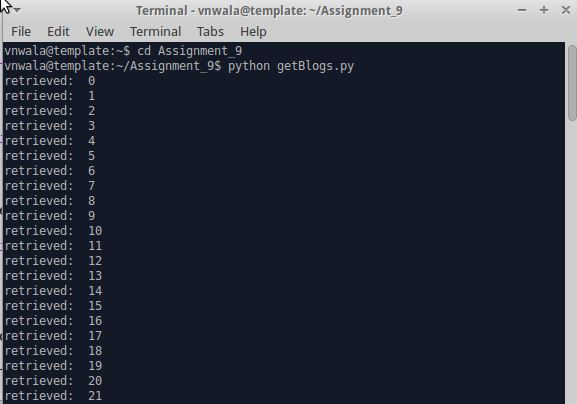
\includegraphics[width=0.75\columnwidth]{getBlogs} % Example image
\end{center}


}

\pythonscript{get500Popular}{Code to get frequent 500 terms and create blogdata}
Note:This code is used for both problem 1 and 5
\newpage
Create a histogram of how many pages each blog has (e.g., 30
blogs with just one page, 27 with two pages, 29 with 3 pages and 
so on).
\pythonscript{getNextPage}{Code to count number of pages in a link}

\problemAnswer{

\begin{center}
Figure 2: getNextPage.py at work (Credits to Alexander Nwala)
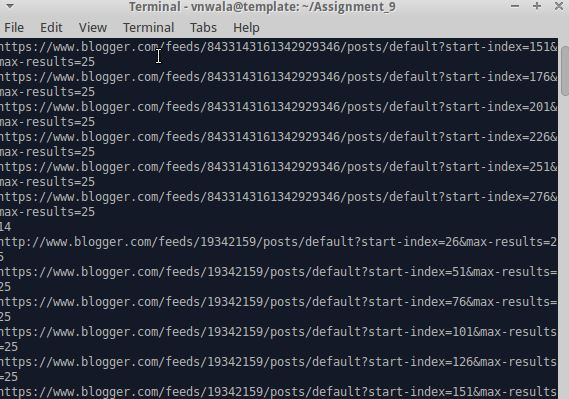
\includegraphics[width=0.75\columnwidth]{getNextPage} % Example image
\end{center}

}

\problemAnswer{

\begin{center}
Figure 3: Histogram of Pages in Blogs
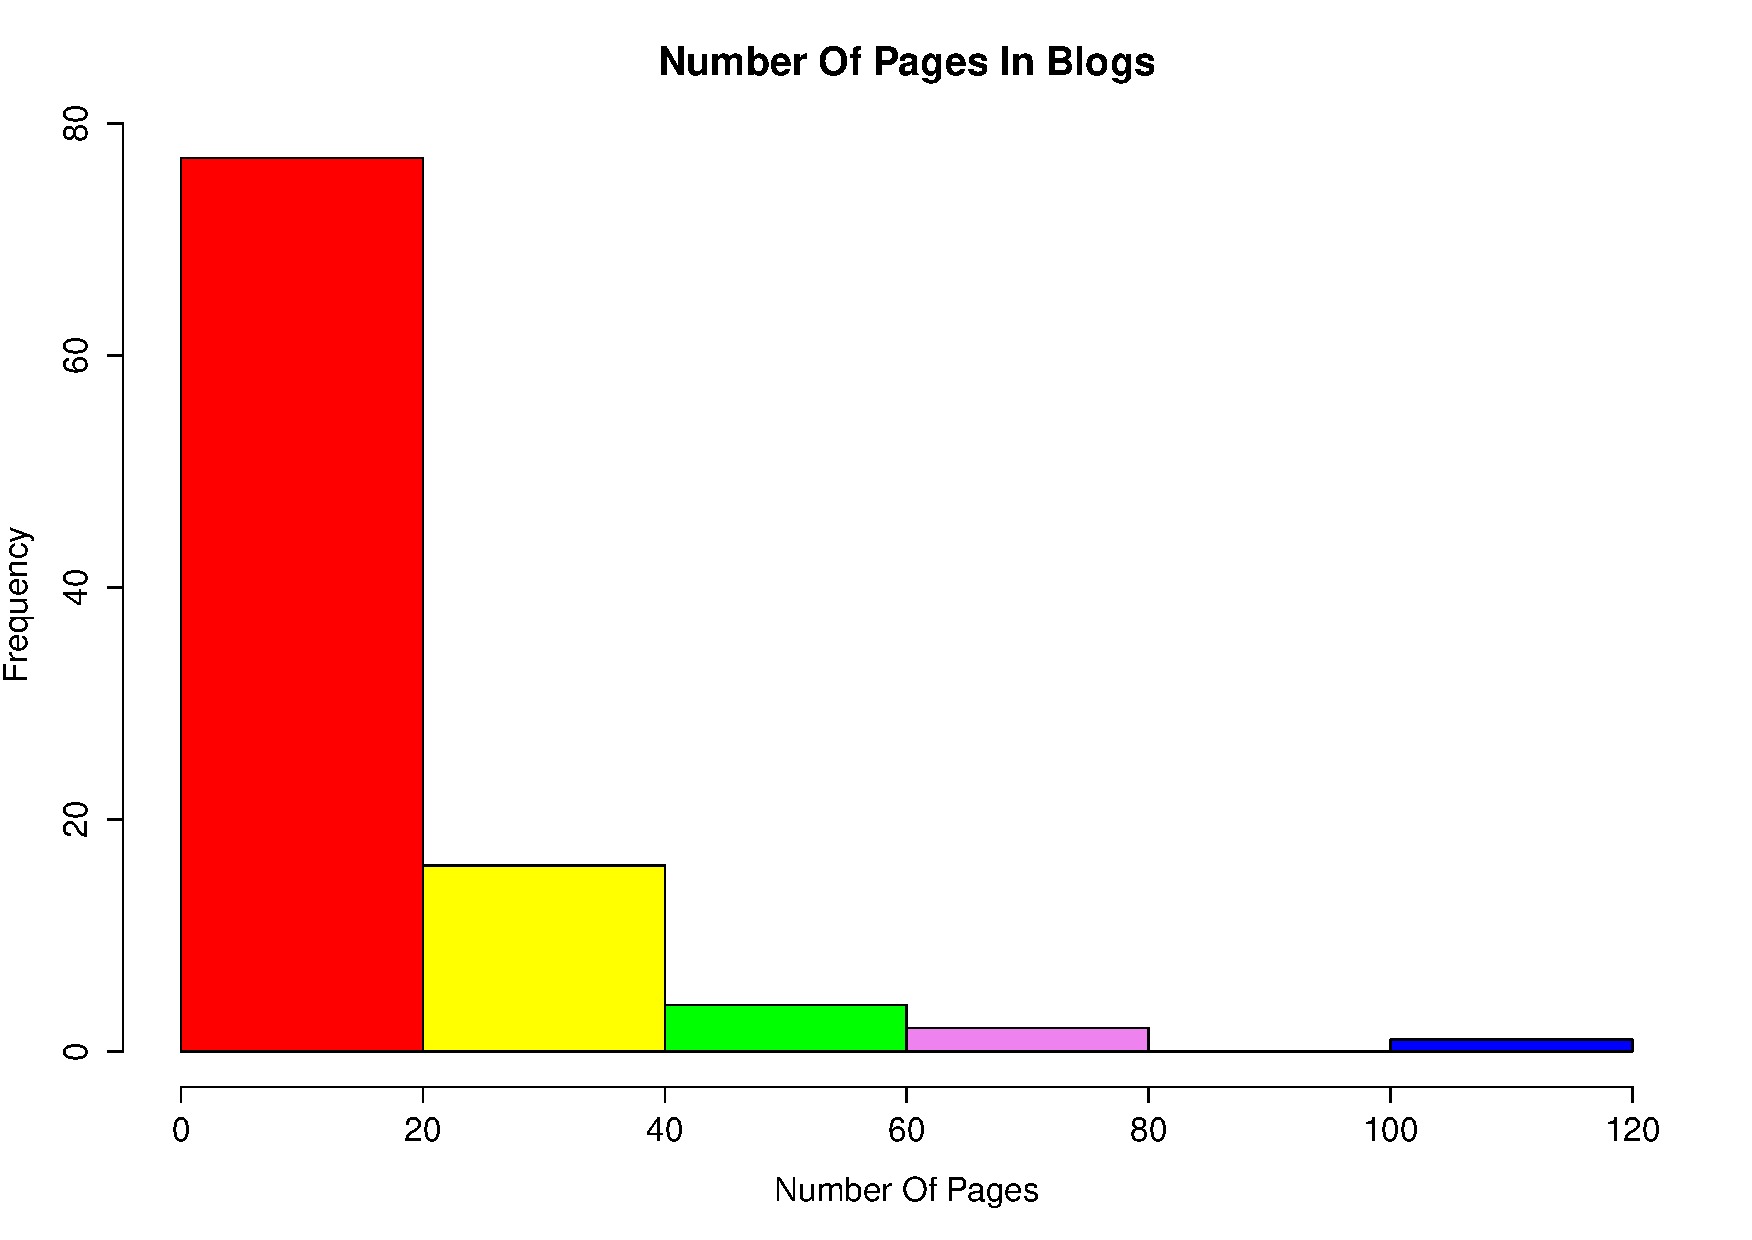
\includegraphics[width=0.75\columnwidth]{pages} % Example image
\end{center}

}  
\end{homeworkProblem}

\newpage
%----------------------------------------------------------------------------------------
%	PROBLEM 2
%----------------------------------------------------------------------------------------

\begin{homeworkProblem}
2.  Create an ASCII and JPEG dendrogram that clusters (i.e., HAC)
the most similar blogs (see slides 12 \& 13).  Include the JPEG in
your report and upload the ascii file to github (it will be too
unwieldy for inclusion in the report).
The ASCII file is saved with the file name ascii.txt 


\pythonscript{ascii}{Code to answer problem 2 to 5}


\problemAnswer{
\begin{center}
Figure 4: Ascii of most similar Blogs 
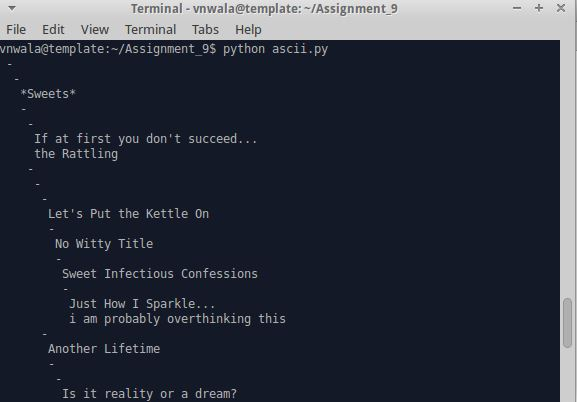
\includegraphics[width=0.75\columnwidth]{ascii} % Example image
\end{center}
}


\problemAnswer{
\begin{center}
Figure 5: Dendogram  for Blog
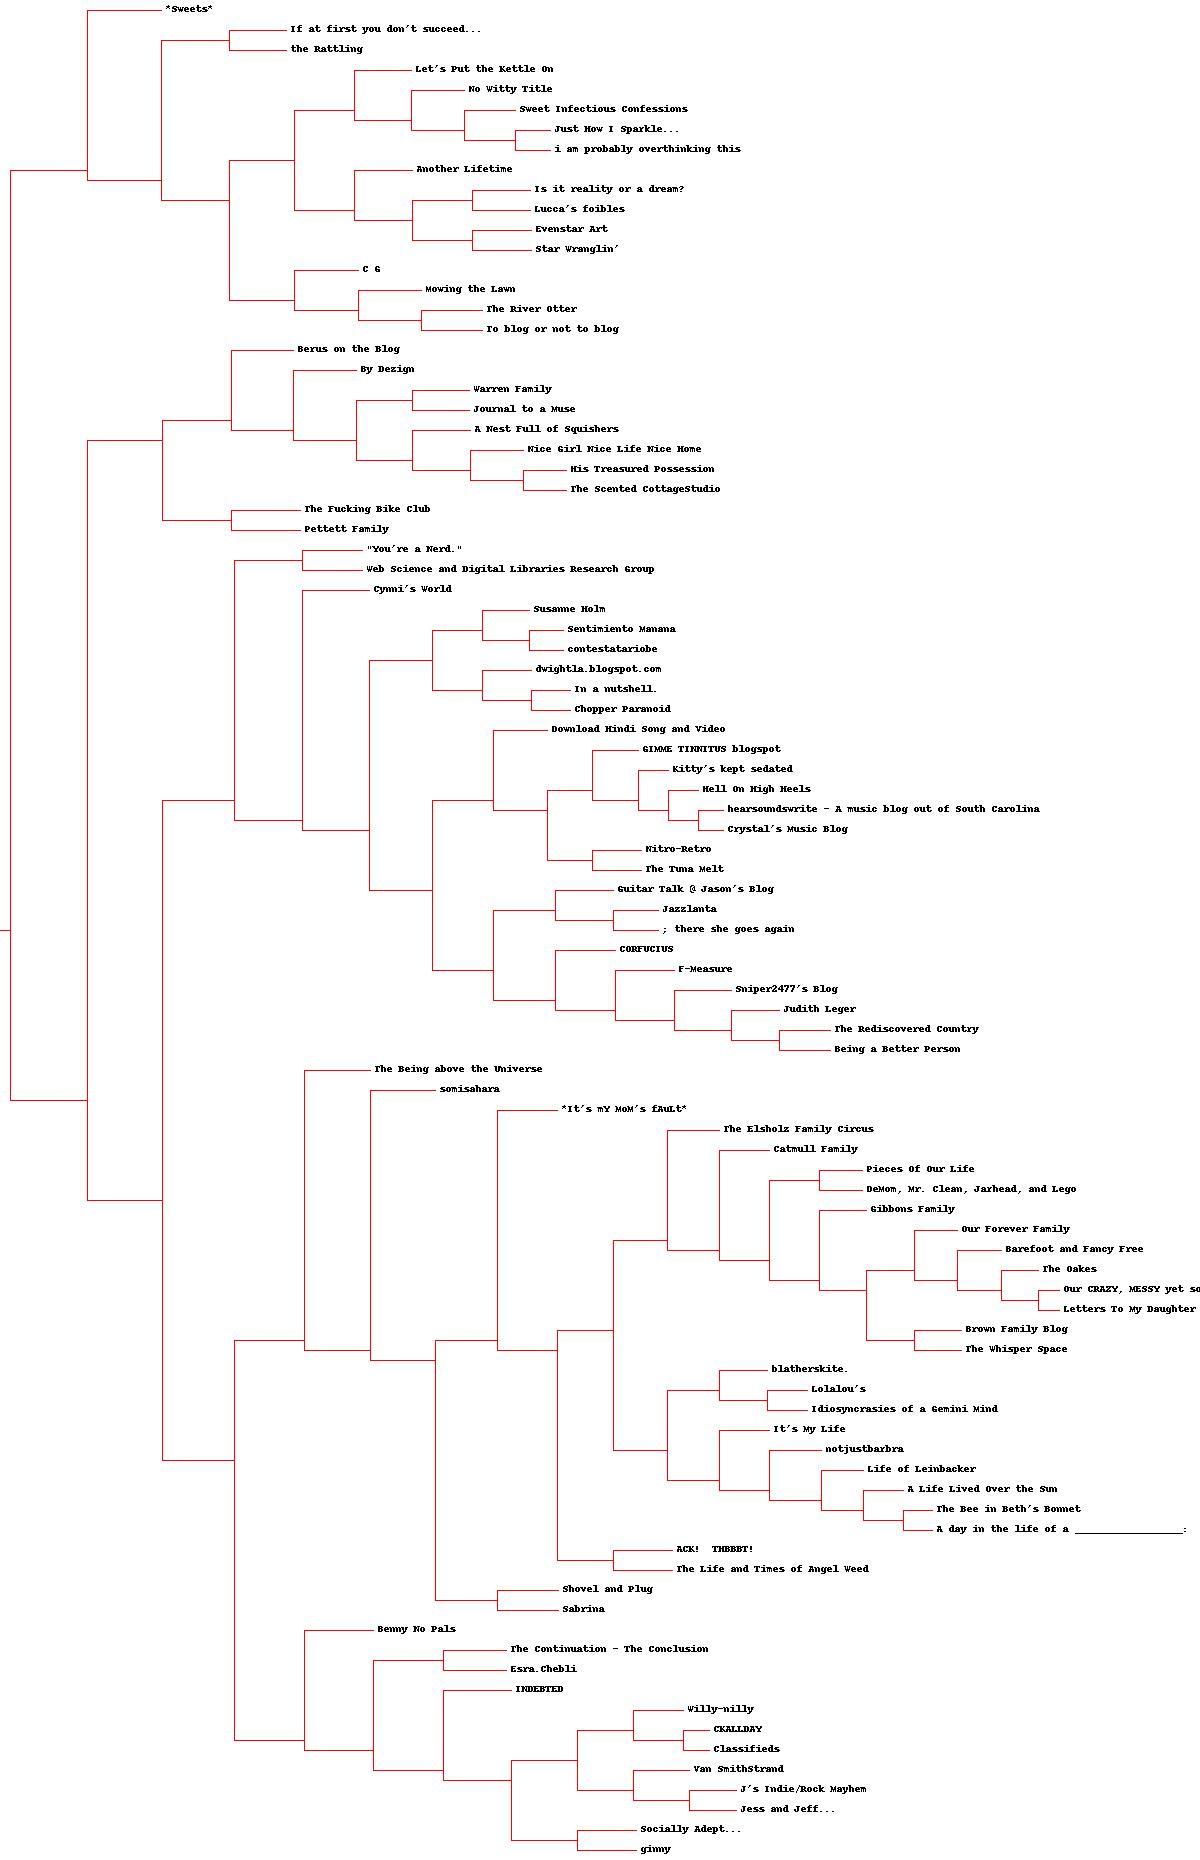
\includegraphics[width=0.75\columnwidth]{blogclust} % Example image
\end{center}


}
\end{homeworkProblem}
\newpage
%----------------------------------------------------------------------------------------
%	PROBLEM 3
%----------------------------------------------------------------------------------------
\begin{homeworkProblem}
3.  Cluster the blogs using K-Means, using k=5,10,20. (see slide 18).
How many interations were required for each value of k?
K = 5 has 8 iterations, k = 10 has 6 iterations while k = 20 has 5 iterations.


\problemAnswer{
\begin{center}
Figure 6: Showing number of iterations for K=5
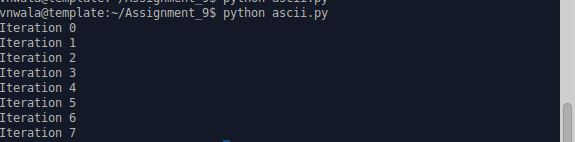
\includegraphics[width=0.75\columnwidth]{k=5} % Example image
\end{center}


}
\problemAnswer{
\begin{center}
Figure 7: Showing number of iterations for K=10
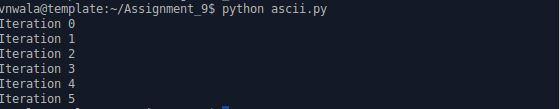
\includegraphics[width=0.75\columnwidth]{k=10} % Example image
\end{center}


}
\problemAnswer{
\begin{center}
Figure 8: Showing number of iterations for K=20
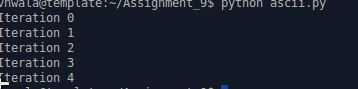
\includegraphics[width=0.75\columnwidth]{k=20} % Example image
\end{center}

}

\end{homeworkProblem}
\newpage
%----------------------------------------------------------------------------------------
%	PROBLEM 4
%----------------------------------------------------------------------------------------


\begin{homeworkProblem}
4.  Use MDS to create a JPEG of the blogs similar to slide 29.  
How many iterations were required?

To create this mds 4 iterations were required.

\problemAnswer{
\begin{center}
Figure 9: MDS JPEG of the Blogs
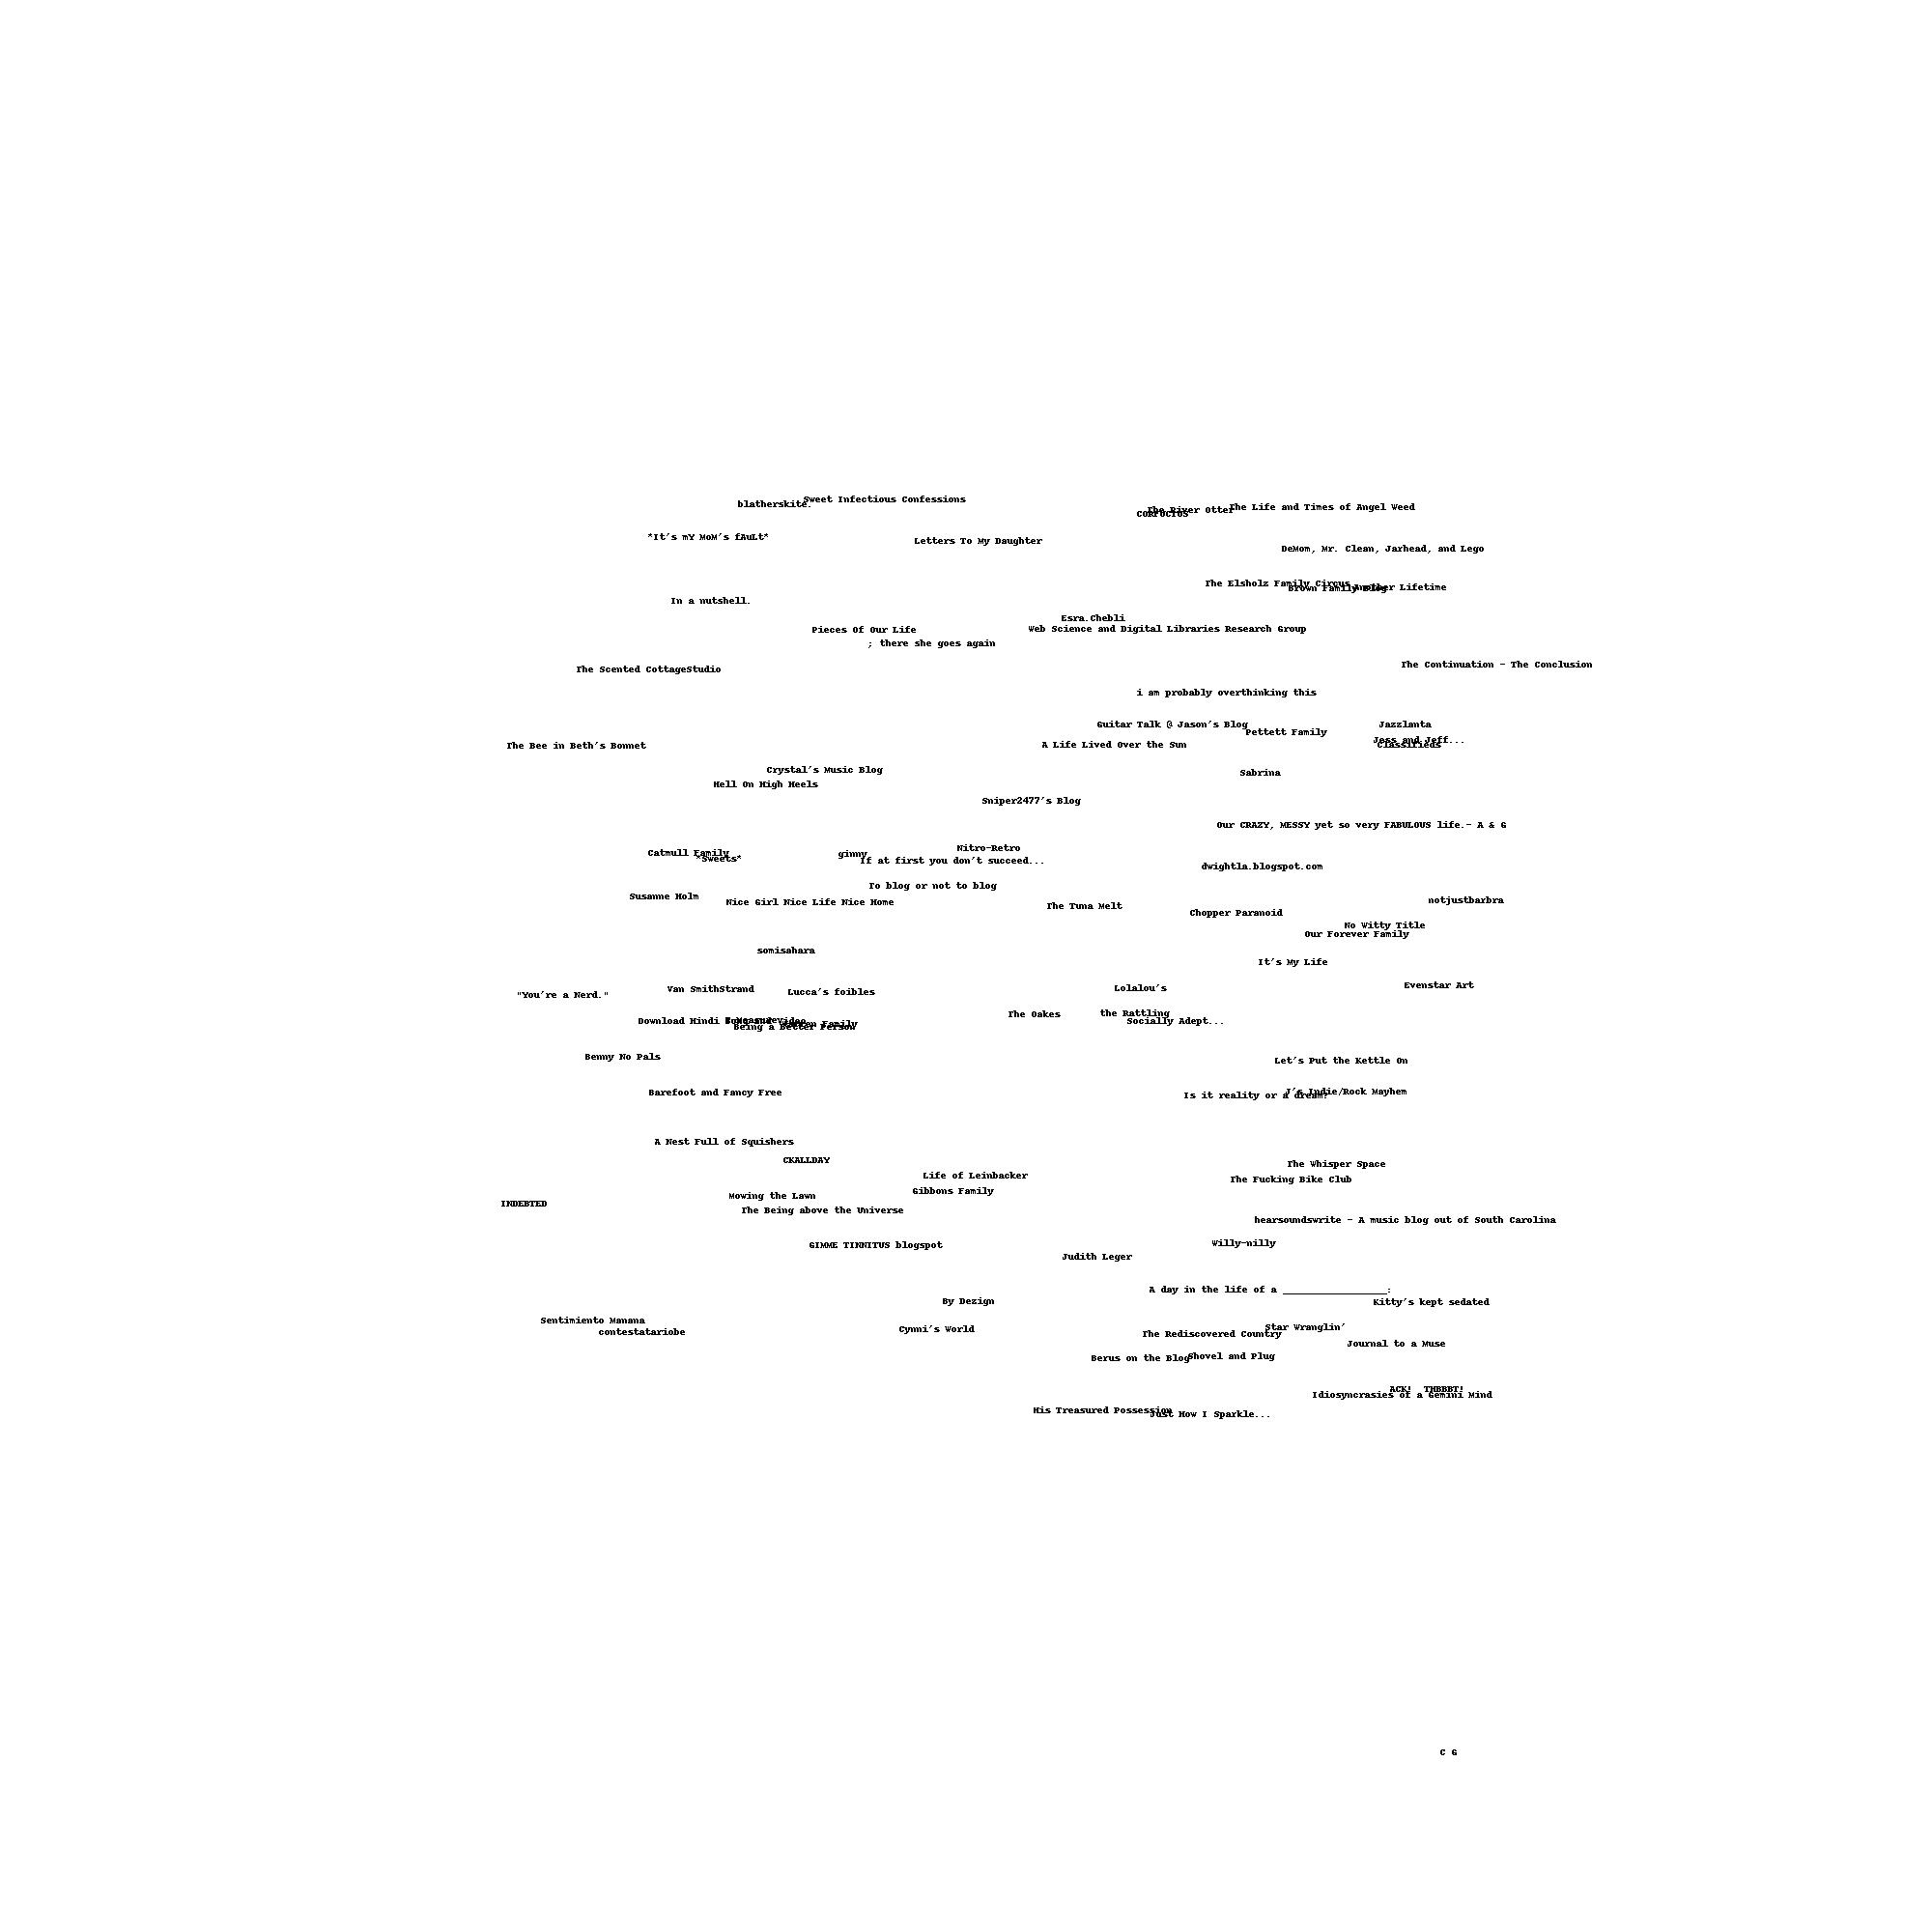
\includegraphics[width=0.75\columnwidth]{blogs2d} % Example image
\end{center}

}
\problemAnswer{
\begin{center}
Figure 10: Showing number of iterations
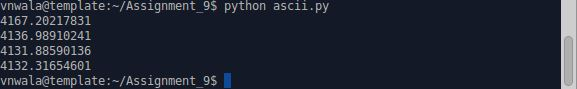
\includegraphics[width=0.75\columnwidth]{mds} % Example image
\end{center}

}
\end{homeworkProblem}

\newpage
%----------------------------------------------------------------------------------------
%	PROBLEM 5
%----------------------------------------------------------------------------------------

\begin{homeworkProblem}
5.  Re-run question 2, but this time with proper TFIDF calculations
instead of the hack discussed on slide 7 (p. 32).  Use the same 500
words, but this time replace their frequency count with TFIDF scores
as computed in assignment \#3.  Document the code, techniques,
methods, etc. used to generate these TFIDF values.  Upload the new
data file to github.

Compare and contrast the resulting dendrogram with the dendrogram
from question \#2.

Note: ideally you would not reuse the same 500 terms and instead
come up with TFIDF scores for all the terms and then choose the top
500 from that list, but I'm trying to limit the amount of work
necessary.

\problemAnswer{
\begin{center}
Figure 11: Showing Dendogram for Blog matrix generated form TFIDF calculations
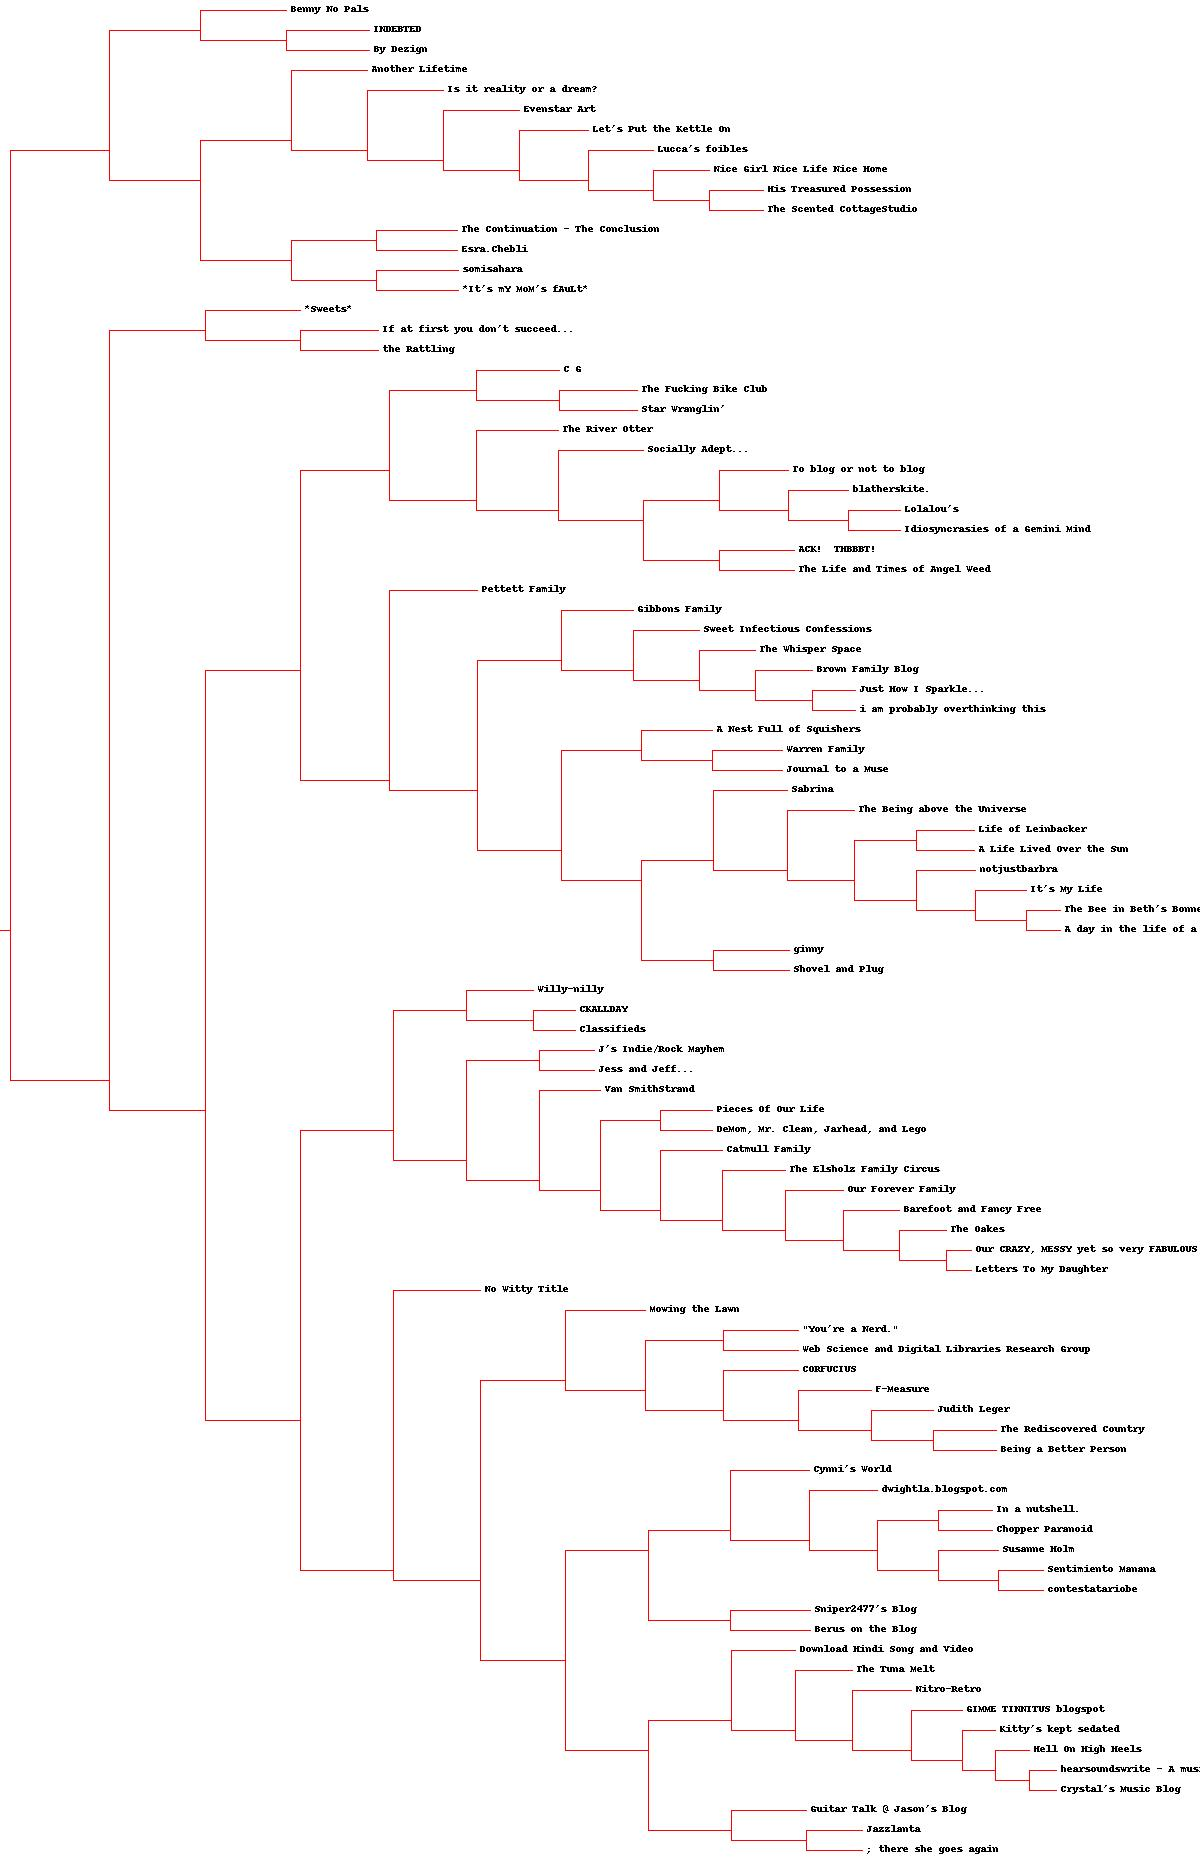
\includegraphics[width=0.75\columnwidth]{blogclustTFIDF} % Example image
\end{center}
}
The function getFeedVector500PopularTFIDF in get500Popular.py is responsible for calculating the TFIDF for the terms (words) in blog. To calculate the TF, number of times a word occurs is divided by the total number of words in that blog ( Line 189 on get500Popular.py). For the IDF the logarithm to the base of two is taken of the division of the total number of words in the entire file (combination of 100 blogs) by the number of times the word of term occurs in the entire file (blog-matrix)( Line 190 and 193 on get500Popular.py). TFIDF is simply a multiplication of both results for a term (word)( Line 194 on get500Popular.py).

Comparing and Contrasting the dendograms generated from TFIDF calculation and those generated from question 2, I observed certain blogs titles appeared in the same cluster in both cases. For example,

``Sweets", ``If at first you don't succeed...", ``the Rattling" appeared in the same cluster in both cases, others who followed the same trend are, ``Willy-nilly",``CKALLDAY",``Classifieds",``Van SmithStrand",``J's Indie/Rock Mayhem", ``Jess and Jeff...", others are, ``You're a Nerd" and ``Web Science and Digital Libraries Research Group", finally ``CORFUCIUS" and ``F-Measure" .
These are some similarites I observed. Also the ASCII file generated in problem 5 is saved with the name asciiTFIDF.txt


\end{homeworkProblem}
\section{Conclusion}
To conclude, I should state that Alexander Nwala was a huge contributor to solving problem 1 and 5.

\newpage
%------------------------------------------------------------------
%  Bibilography
%------------------------------------------------------------------
\bibliographystyle{plain}
\bibliography{assignment_9}
\cite{*}
%----------------------------------------------------------------------------------------

\end{document}
